  \documentclass[11pt,a4paper]{article}

  % ============================================================
  %  Delegação Capacitária com Profundidade Limitada (CASL)
  %  Modelo formal + enforcement por Row-Level Security
  %  Patria Technology — patria-erp
  % ============================================================

  \usepackage[utf8]{inputenc}
  \usepackage[T1]{fontenc}
  \usepackage[brazil]{babel}
  \usepackage{amsmath,amssymb,amsthm}
  \usepackage{mathtools}
  \usepackage{stmaryrd}
  \usepackage{enumitem}
  \usepackage{hyperref}
  \usepackage{graphicx}
  \usepackage{tikz}
  \usetikzlibrary{trees,positioning,fit,backgrounds,calc,arrows.meta}

  \hypersetup{colorlinks=true,linkcolor=blue!50!black,urlcolor=blue!50!black}

  \newtheorem{theorem}{Teorema}
  \newtheorem{lemma}[theorem]{Lema}
  \newtheorem{corollary}[theorem]{Corolário}
  \newtheorem{proposition}[theorem]{Proposição}
  \theoremstyle{definition}
  \newtheorem{definition}[theorem]{Definição}
  \newtheorem{remark}[theorem]{Observação}

  \newcommand{\R}{\mathcal{R}}
  \newcommand{\ext}[1]{\llbracket #1 \rrbracket}
  \newcommand{\Subj}{\mathcal{S}}
  \newcommand{\Act}{\mathcal{A}}
  \newcommand{\tenant}{\texttt{tenantId}}
  \newcommand{\dep}{\delta}
  \newcommand{\NN}{\mathbb{N}_0}
  \newcommand{\F}{\mathcal{F}}
  \newcommand{\dS}{\mathrm{dS}}

  \title{\textbf{Delegação Capacitária com Profundidade Limitada}\\[2mm]
  \large Um modelo de controle de acesso distribuído sobre CASL,\\
  com grafo de delegação, intensidade de propagação,\\
  e \emph{enforcement} por \emph{Row-Level Security}}
  \author{Patria Technology --- \texttt{patria-erp}}
  \date{Maio de 2026}

  \begin{document}
  \maketitle

  \begin{abstract}
  Modelamos o controle de acesso do \texttt{patria-erp} como \emph{delegação
  capacitária}: autoridades intrínsecas (o operador da plataforma, que tudo
  vê; e cada \emph{tenant}, com controle total dos próprios recursos) emitem
  \emph{capacidades} que fluem por um \textbf{grafo de delegação} dirigido
  finito --- não uma árvore, e nem precisa ser acíclico: um concedente pode
  autorizar \emph{diretamente} qualquer principal, e a segurança vem da
  atenuação ($\dep$ como energia bem-fundada), não da estrutura do grafo.
  Duas teses estruturam o modelo: (i) \textbf{desacoplar o \emph{tenant}},
  que deixa de ser eixo especial e vira apenas \emph{uma condição} dentro de
  uma capacidade; e (ii) dotar cada concessão de uma \textbf{intensidade}
  $\dep$ --- a \emph{profundidade de propagação} --- que limita quantas
  re-delegações ela admite ($\dep=0$: o destinatário usa mas não compartilha;
  $\dep=k$: re-delegável por mais $k$ saltos, decrementando; $\dep=\infty$:
  irrestrito). Mostramos que a delegação é uma \emph{atenuação} (condição
  $\subseteq$ e $\dep$ decrementado), o que garante não-escalada de
  privilégio por construção, e que o \emph{enforcement} se reduz a empurrar a
  \emph{união} das condições detidas para o \texttt{where} das consultas
  (\emph{pushdown}), realizado por uma extensão do Prisma Client. Um ponto
  operacional central: $\dep$ é verificado no \textbf{ato de delegar}, não na
  leitura. Por fim, modelamos o \textbf{ciclo de vida} de cada concessão como
  uma máquina de estados (\textsf{active}/\textsf{suspended}/\textsf{revoked}/
  \textsf{expired}): a revogação \emph{cascateia} pela cadeia de delegação e a
  expiração se propaga sozinha pelo invariante de atenuação
  ($\tau_{\text{filho}}\le\tau_{\text{pai}}$). Por baixo de tudo,
  caracterizamos o sistema como um \textbf{fluxo monótono sobre um reticulado
  booleano} --- semianel idempotente $(2^{\R},\cup,\cap)$ para a autorização,
  operador de atenuação deflacionário $T\preceq\mathrm{id}$ para a delegação ---
  do que os teoremas (não-escalada, propagação limitada, fail-closed) seguem
  como corolários. A profundidade $\dep$, por sua vez, é a iteração do operador
  de \emph{propagação} $P\succeq\mathrm{id}$ (dual da atenuação) sobre os
  conjuntos de principals, com $\dep=\infty$ no seu \emph{menor} ponto fixo
  $\mu P$ (fecho transitivo). O Apêndice~\ref{ap:plano} traz o plano de
  implementação.
  \end{abstract}

  \tableofcontents
  \bigskip

  % ============================================================
  \section{Introdução e motivação}
  % ============================================================

  A Patria opera uma plataforma multi-organização. Cada cliente (um
  \emph{tenant}) controla os próprios cadastros, vendas, alunos, mensalidades;
  a Patria, como operadora, precisa \emph{ver e operar} centralmente sobre os
  clientes; e dentro de cada cliente há níveis de acesso. Isso é
  \emph{delegação}: a autoridade flui de quem a tem para quem a recebe.

  Duas decisões de projeto. Primeiro, \textbf{o \emph{tenant} não é especial}:
  em vez de um ``piso'' fixo (\texttt{where:\{tenantId\}}) espalhado por
  centenas de \emph{services}, o isolamento é apenas a condição
  $c_t=(\tenant=t)$ embutida nas capacidades. Segundo --- e é o ponto que
  distingue este modelo --- toda concessão carrega uma \textbf{intensidade
  $\dep$} que limita a sua re-delegação. Sem isso, dar a um usuário acesso a
  dados de outro \emph{tenant} contaminaria toda a cadeia abaixo dele; com
  $\dep=0$, o acesso fica \emph{só naquele usuário}.

  Por fim, a estrutura de delegação \textbf{não é uma árvore} --- e nem precisa
  ser acíclica: um \emph{tenant} pode conceder \emph{diretamente} a um usuário,
  e nada impede um ciclo (Financeiro $\to$ João $\to$ Grupo $\to$ Financeiro).
  O substrato é um \emph{grafo dirigido finito} de concessões; a segurança não
  vem da aciclicidade, mas da \textbf{atenuação} (Seção~\ref{sec:dag}).

  % ============================================================
  \section{Preliminares}
  % ============================================================

  \begin{definition}[Linhas e condições]
  Seja $\R$ o universo de todas as linhas. Cada $r\in\R$ tem atributos
  ($r.\tenant$, $r.\texttt{id}$, \dots). Uma \emph{condição} $c$ é um predicado
  $c:\R\to\{\bot,\top\}$, identificado ao seu \emph{extent}
  $\ext{c}=\{r\in\R:c(r)\}\subseteq\R$. As condições formam a álgebra booleana
  $(2^{\R},\cap,\cup,\setminus,\varnothing,\R)$ --- as \emph{MongoQuery} do CASL.
  \end{definition}

  \begin{remark}[Identificação semântica --- nunca sintática]\label{rem:extent}
  Toda \emph{MongoQuery} é identificada ao seu \emph{extent}: os construtores
  sintáticos do CASL mapeiam-se nas operações da álgebra,
  \[
    \ext{\{\texttt{AND}{:}[c_1,c_2]\}}=\ext{c_1}\cap\ext{c_2},\quad
    \ext{\{\texttt{OR}{:}[c_1,c_2]\}}=\ext{c_1}\cup\ext{c_2},\quad
    \ext{\{\texttt{NOT}{:}c\}}=\R\setminus\ext{c}.
  \]
  Raciocinamos sempre sobre \emph{conjuntos de linhas}, jamais sobre a forma
  da query --- duas queries sintaticamente distintas com o mesmo extent são,
  para nós, a \emph{mesma} condição. (Isto não trivializa a implementação: o
  teste de inclusão $\subseteq$ no \emph{grant-check} é conservador justamente
  porque decidir $\subseteq$ sintaticamente é incompleto; ver
  Seção~\ref{sec:enf}.)
  \end{remark}

  Fixamos \emph{subjects} $\Subj$ (\texttt{Customer}, \texttt{Student}, \dots),
  \emph{ações} $\Act=\{\texttt{create},\texttt{read},\texttt{update},
  \texttt{delete}\}$ ($\texttt{manage}=\bigvee\Act$) e o curinga \texttt{all}.

  \begin{definition}[Capacidade]\label{def:cap}
  Uma \emph{capacidade} é uma tupla
  \[
    \kappa=(a,\,s,\,c,\,\iota,\,\dep), \qquad
    \dep\in\NN\cup\{\infty\},
  \]
  com ação $a$, subject $s$, condição $c$, \emph{flag} de inversão $\iota$
  ($\iota{=}1$ é uma \emph{proibição}, \texttt{cannot}) e \emph{profundidade de
  propagação} (intensidade) $\dep$. Informalmente, $\kappa$ autoriza (ou nega,
  se $\iota{=}1$) $a$ sobre $s$ nas linhas de $\ext{c}$, e admite ser
  re-delegada por mais $\dep$ saltos.
  \end{definition}

  % ============================================================
  \section{Autorização de um principal}
  % ============================================================

  Seja $P$ o conjunto de \emph{principals} (operador, donos de \emph{tenant},
  perfis, usuários). Cada principal \emph{detém} um conjunto de capacidades
  $\mathrm{Hold}(p)$ (Seção~\ref{sec:dag}). Para um par fixo $(s,a)$, a
  autorização efetiva é a \textbf{união} dos grants menos as proibições:
  \[
    E_p(s,a)\;=\;
    \Bigl(\bigcup_{\substack{\kappa\in\mathrm{Hold}(p)\\ \iota_\kappa=0,\ \kappa\vdash(s,a)}}\ext{c_\kappa}\Bigr)
    \ \setminus\
    \Bigl(\bigcup_{\substack{\kappa\in\mathrm{Hold}(p)\\ \iota_\kappa=1,\ \kappa\vdash(s,a)}}\ext{c_\kappa}\Bigr),
  \]
  onde $\kappa\vdash(s,a)$ significa que $\kappa$ casa o subject e a ação
  (com \texttt{manage}/\texttt{all} como curingas).

  \begin{remark}[A intensidade não entra aqui]
  $E_p$ \emph{não} depende de $\dep$: a profundidade governa a \emph{delegação}
  (Seção~\ref{sec:dag}), não a avaliação. Quem detém uma capacidade a exerce
  plenamente, qualquer que seja o seu $\dep$ restante. Isso é o que torna o
  \emph{enforcement} barato (Seção~\ref{sec:enf}).
  \end{remark}

  \begin{remark}[União, não interseção]
  Compor grants com interseção seria um erro: ``ler onde \texttt{org}$=A$'' e
  ``ler onde \texttt{org}$=B$'' devem autorizar $A\cup B$. Só as proibições
  subtraem.
  \end{remark}

  \begin{proposition}[\emph{Deny-overrides} --- a proibição sempre vence]
  \label{prop:deny}
  A escolha de política está \emph{embutida} na diferença de conjuntos: para
  toda linha $r$,
  \[
    r\in E_p(s,a)\iff
    \bigl(\exists\,\text{grant }g:\ r\in\ext{c_g}\bigr)\ \wedge\
    \bigl(\nexists\,\text{proibição }d:\ r\in\ext{c_d}\bigr).
  \]
  Uma proibição domina \emph{qualquer} grant sobre a mesma linha,
  independentemente de ``especificidade'' ou ordem. Assim, grant
  $\{\texttt{customerId}{=}5\}$ com proibição $\{\tenant{=}A\}$ (e $5\in A$)
  resulta $\varnothing$: a proibição vence. O sistema é, por definição,
  \textbf{deny-overrides} --- declarado aqui para remover ambiguidade. (Casa
  com a semântica do CASL, onde \texttt{cannot} sobrepõe \texttt{can}.)
  \end{proposition}

  % ============================================================
  \section{O grafo de delegação e a atenuação}\label{sec:dag}
  % ============================================================

  \begin{definition}[Autoridades intrínsecas]
  Duas fontes de autoridade não derivam de ninguém:
  \begin{itemize}[nosep]
    \item o \textbf{operador} $\Omega$ detém $(\texttt{manage},\texttt{all},
          \top,0,\infty)$ --- vê e faz tudo, com re-delegação irrestrita;
    \item o \textbf{dono do \emph{tenant}} $t$ detém
          $(\texttt{manage},\texttt{all},(\tenant{=}t),0,\infty)$ --- controle
          total dos próprios recursos.
  \end{itemize}
  \end{definition}

  \begin{definition}[Grafo de delegação]\label{def:dag}
  Um \emph{grafo de delegação} é um \emph{grafo dirigido finito} (não
  necessariamente acíclico) cujos vértices são principals e cujas arestas
  $u\xrightarrow{\kappa}w$ representam ``$u$ concede a capacidade $\kappa$ a
  $w$''. $w$ é \emph{qualquer} principal --- sem exigência de árvore, de
  vizinhança ou de aciclicidade.
  \end{definition}

  \begin{definition}[Concessão válida / atenuação]\label{def:att}
  A aresta $u\xrightarrow{\kappa}w$ é \emph{válida} se existe
  $\kappa_0\in\mathrm{Hold}(u)$ tal que
  \[
    \ext{c_\kappa}\subseteq\ext{c_{\kappa_0}},\quad
    \kappa\vdash(s,a)\Rightarrow\kappa_0\vdash(s,a),\quad
    \iota_\kappa=\iota_{\kappa_0},\quad
    \dep_{\kappa_0}\ge 1,\quad
    \dep_\kappa\le \dep_{\kappa_0}-1,\quad
    \tau_\kappa\le\tau_{\kappa_0},
  \]
  com a convenção $\infty-1=\infty$. Isto é, $u$ só concede o que detém,
  \emph{nunca ampliando} a condição, \emph{sempre decrementando} a
  profundidade e \emph{nunca estendendo} a validade $\tau$ (expiração,
  Seção~\ref{sec:lifecycle}). Em particular $\dep_{\kappa_0}=0$ proíbe qualquer
  concessão.
  \end{definition}

  \begin{definition}[Capacidades detidas]
  $\mathrm{Hold}(p)$ é o menor conjunto que contém as capacidades intrínsecas
  de $p$ (se $p$ é $\Omega$ ou dono) e toda $\kappa$ tal que existe uma aresta
  válida $u\xrightarrow{\kappa}p$.
  \end{definition}

  % ------------------------------------------------------------
  \subsection{A intensidade $\dep$: profundidade de propagação}
  % ------------------------------------------------------------

  Por construção (Definição~\ref{def:att}), uma capacidade emitida com
  profundidade $\dep$ admite cadeias de re-delegação de comprimento no máximo
  $\dep$:
  \[
    \dep \xrightarrow{\text{1 salto}} \dep-1 \xrightarrow{} \cdots \xrightarrow{} 0
    \ (\text{não re-delegável}).
  \]
  \begin{itemize}[nosep]
    \item $\dep=0$: o destinatário \emph{usa} a capacidade, mas não a passa a
          ninguém. É o caso do ``dar acesso sem permitir compartilhar''.
    \item $\dep=k$: re-delegável por mais $k$ saltos; cada salto decrementa.
    \item $\dep=\infty$: irrestrito (o comportamento legado, sem limite).
  \end{itemize}

  \begin{lemma}[$\dep$ é uma energia bem-fundada $\Rightarrow$ ciclos são inofensivos]
  \label{lem:energy}
  Como toda aresta válida \emph{estritamente} decrementa a profundidade
  ($\dep_\kappa\le\dep_{\kappa_0}-1$, Definição~\ref{def:att}), $\dep$ é um
  \emph{variante bem-fundado} sobre as cadeias de re-delegação: qualquer
  caminho de concessões com $\dep$ finito tem comprimento $\le\dep$ e termina.
  \textbf{Logo a aciclicidade do grafo é dispensável} --- um ciclo
  $u\to v\to\cdots\to u$ apenas faz $\dep$ cair a cada volta até $0$, quando a
  propagação para. A terminação (e a não-escalada) vem da atenuação, não da
  estrutura do grafo. Só $\dep=\infty$ ignora a energia; reserve-o às
  autoridades intrínsecas.
  \end{lemma}

  \begin{figure}[h]
  \centering
  \begin{tikzpicture}[
      every node/.style={font=\small},
      P/.style={draw,circle,inner sep=2pt,fill=blue!6,minimum size=8mm},
      dlbl/.style={midway,font=\scriptsize,text=black!70,align=center},
      >={Stealth[round]},
    ]
    \node[P] (op) {$\Omega$};
    \node[P, below=14mm of op] (ad) {A};
    \node[P, below left=16mm and 10mm of ad] (u1) {$u_1$};
    \node[P, below right=16mm and 10mm of ad] (u2) {$u_2$};
    \node[P, below=14mm of u1] (u3) {$u_3$};

    % delegação intrínseca e cross-tenant com profundidade
    \draw[->] (op) -- (ad) node[dlbl,right]{cross-tenant\\ $(\tenant{=}B,\ \dep{=}1)$};
    \draw[->] (ad) -- (u1) node[dlbl,left]{$\dep{=}0$};
    \draw[->,dashed,gray] (u1) -- (u3) node[dlbl,left]{\textcolor{red!70!black}{bloqueada}\\ $\dep{=}0$};
    \draw[->] (ad) -- (u2) node[dlbl,right]{interno A\\ $(\tenant{=}A,\ \dep{=}0)$};
  \end{tikzpicture}
  \caption{Grafo de delegação (dirigido finito, não árvore, ciclos permitidos). $\Omega$ concede a $A$ uma
  capacidade cross-\emph{tenant} ($\tenant{=}B$) com $\dep{=}1$; $A$ pode
  re-delegá-la \emph{uma} vez (a $u_1$, com $\dep{=}0$), mas $u_1$ \emph{não}
  pode repassá-la (aresta bloqueada). $A$ também concede algo interno
  diretamente a $u_2$. As arestas são explícitas --- $A$ alcança $u_1,u_2$
  diretamente, sem intermediários obrigatórios.}
  \label{fig:dag}
  \end{figure}

  % ============================================================
  \section{Invariantes de segurança}
  % ============================================================

  \begin{theorem}[Não-escalada por atenuação]\label{thm:noesc}
  Para todo $p$ e toda $\kappa\in\mathrm{Hold}(p)$, existe uma autoridade
  intrínseca $\kappa_0$ e uma cadeia de arestas válidas de sua origem até $p$
  tais que $\ext{c_\kappa}\subseteq\ext{c_{\kappa_0}}$. Logo
  \[
    E_p(s,a)\ \subseteq\ \bigcup_{\kappa_0\ \text{(raiz que alcança }p)}\ext{c_{\kappa_0}} .
  \]
  Nenhum principal acessa uma linha que nenhuma autoridade intrínseca em sua
  cadeia podia conceder.
  \end{theorem}
  \begin{proof}
  Indução no comprimento da cadeia de delegação. Caso base: capacidade
  intrínseca. Passo: a Definição~\ref{def:att} exige
  $\ext{c_\kappa}\subseteq\ext{c_{\kappa_0}}$ a cada aresta; a inclusão é
  transitiva. A cota de $E_p$ segue por monotonicidade da união.
  \end{proof}

  \begin{theorem}[Propagação limitada]\label{thm:bounded}
  Uma capacidade emitida com profundidade $\dep$ só pode aparecer (atenuada)
  ao fim de cadeias de re-delegação de comprimento $\le\dep$. Em particular,
  $\dep=0\Rightarrow$ não re-delegável: ela permanece exclusivamente no
  destinatário direto.
  \end{theorem}
  \begin{proof}
  Cada aresta válida decrementa $\dep$ em pelo menos 1 e exige $\dep_{\kappa_0}
  \ge1$ (Definição~\ref{def:att}); uma cadeia de comprimento $\ell$ requer
  $\dep\ge\ell$. Para $\dep=0$ não há aresta de saída possível.
  \end{proof}

  \begin{corollary}[Compartilhamento controlado]
  Conceder uma capacidade cross-\emph{tenant} com $\dep=0$ garante que o
  destinatário a exerce mas ninguém abaixo dele a herda --- exatamente ``dar
  acesso sem propagar''. Com $\dep=k$, a difusão é confinada à vizinhança de
  re-delegação de raio $k$.
  \end{corollary}

  \begin{remark}[Fail-closed $=$ união vazia]
  Se nenhum grant detido casa $(s,a)$, então $E_p(s,a)=\varnothing$: acesso
  negado. É o \emph{bottom} da álgebra, uniforme --- sem piso de tenant
  especial.
  \end{remark}

  % ============================================================
  \section{O tenant como caso particular (desacoplamento)}
  % ============================================================

  \begin{corollary}[Isolamento de tenant]
  Um usuário comum da organização $t$ só detém capacidades atenuadas da
  capacidade intrínseca do dono, todas com $\ext{c}\subseteq\ext{\tenant{=}t}$.
  Logo $E_p\subseteq\{r:r.\tenant=t\}$: nenhuma linha de outro \emph{tenant}
  aparece, \emph{sem} regra especial. Um vazamento cross-\emph{tenant} só
  ocorre por uma aresta de concessão explícita (auditável), cuja difusão é
  exatamente governada por $\dep$.
  \end{corollary}

  O operador $\Omega$, detendo $\top$, enxerga todos os \emph{tenants} --- ``eu,
  no topo, vejo tudo''. O \emph{tenant} foi reduzido a uma condição.

  % ============================================================
  \section{Caracterização algébrica}\label{sec:algebra}
  % ============================================================

  Tudo o que precede é, na verdade, \emph{um fluxo monótono sobre um reticulado
  booleano}. Tornar isso explícito entrega vários teoremas quase de graça.

  \begin{definition}[O dioid das condições]
  $(2^{\R},\oplus,\otimes)$ com $\oplus:=\cup$ e $\otimes:=\cap$ é um
  \emph{semianel idempotente comutativo} (dioid): $\oplus$ é associativa,
  comutativa, \emph{idempotente} ($a\oplus a=a$), com neutro $\varnothing$;
  $\otimes$ idem, com neutro $\R$; e $\otimes$ distribui sobre $\oplus$. A
  \emph{ordem canônica} $a\preceq b\iff a\oplus b=b$ coincide com $\subseteq$.
  Com o complemento $\neg$, é a álgebra booleana completa
  $(2^{\R},\cup,\cap,\neg,\varnothing,\R)$ --- um \emph{reticulado completo}.
  \end{definition}

  \begin{remark}[Autorização é uma expressão do dioid]
  A Seção~3 é, literalmente, álgebra do semianel:
  \[
    E_p(s,a)=\Bigl(\bigoplus_{g}\ext{c_g}\Bigr)\otimes
            \neg\Bigl(\bigoplus_{n}\ext{c_n}\Bigr),
  \]
  soma dos grants vezes o complemento da soma das proibições. O
  \emph{pushdown} (Seção~\ref{sec:enf}) é apenas avaliar essa expressão.
  \end{remark}

  \begin{definition}[Delegação é um operador monótono deflacionário]
  Cada aresta de delegação induz $T:2^{\R}\to2^{\R}$ com
  \[
    x\preceq y\Rightarrow T(x)\preceq T(y)\quad(\text{monótono}),\qquad
    T(x)\preceq x\quad(\text{deflação: }T\preceq\mathrm{id}).
  \]
  A condição de atenuação $\ext{c_\kappa}\subseteq\ext{c_{\kappa_0}}$
  (Definição~\ref{def:att}) \emph{é} exatamente $T\preceq\mathrm{id}$.
  \end{definition}

  \paragraph{Dois operadores duais (a distinção que importa).}
  A delegação tem \emph{dois} lados, e é tentador --- mas incorreto --- fundir
  os dois. A \textbf{atenuação} $T\preceq\mathrm{id}$ (deflacionária, sobre os
  extents $2^{\R}$) governa \emph{o que}: o extent só encolhe. A
  \textbf{propagação} $P$ governa \emph{quem detém}: sobre o reticulado
  completo $2^{\hat P}$ dos conjuntos de principals,
  \[
    P(H)=H\cup\{\,w:\exists\,u\in H,\ \text{aresta válida }u\to w\,\},
    \qquad P\succeq\mathrm{id}\ (\text{inflacionária}),\ \text{monótona}.
  \]

  \paragraph{Os resultados de graça.}
  \begin{itemize}[nosep,leftmargin=1.3em]
    \item \textbf{Profundidade $=$ iteração da propagação $P$ (não de $T$).}
          Re-delegar por $\dep$ saltos é $P^{\dep}$. A intensidade $\dep=k$ é
          o $k$-ésimo aproximante $P^k(\{\mathrm{orig}\})$ (reach em $\le k$
          saltos); $\dep=\infty$ é o \textbf{menor ponto fixo}
          $\mu P=\bigsqcup_{n}P^n(\{\mathrm{orig}\})$ (Kleene \emph{de baixo})
          --- o fecho transitivo da delegação válida. É um $\mu P$
          \emph{ascendente} sobre quem-detém, \emph{não} um $\nu T$
          descendente sobre extents: as duas ideias não se identificam.
    \item \textbf{Não-escalada $=$ monotonicidade de $T$.} $p\mapsto E_p$ é um
          morfismo monótono da floresta de \emph{derivação} (acíclica por
          atenuação, mesmo que o grafo de delegação tenha ciclos), ordenada
          por derivação, para
          $(2^{\R},\preceq)$. O Teorema~\ref{thm:noesc} é a imagem da ordem.
    \item \textbf{Composição.} Operadores monótonos deflacionários são
          fechados sob $\circ$: a autoridade ao longo de um caminho é
          $T_{e_1}\circ\cdots\circ T_{e_k}$, ainda monótona e deflacionária.
          Cadeias compõem sem sair da classe.
    \item \textbf{Fail-closed $=$ zero.} Ausência de grant $=$ soma vazia $=$
          $\varnothing$ $=$ neutro de $\oplus$. Negar é o zero do semianel
          (Teorema~\ref{thm:bounded} e a Observação de fail-closed).
    \item \textbf{Auditoria por ordem parcial.} $\mathrm{Hold}(p)$ e a floresta
          de derivação são \emph{posets} sob ``derivado-de''; a revogação é o
          \emph{fecho para baixo} (downset), uma operação monótona; expirar/
          revogar só decresce $E_p$ --- a FSM (Seção~\ref{sec:lifecycle}) é um
          fluxo monótono.
  \end{itemize}

  \begin{remark}
  Os teoremas das seções anteriores deixam de ser fatos isolados: são
  corolários de ``$(2^{\R},\cup,\cap)$ é um dioid e a delegação é um operador
  monótono $\preceq\mathrm{id}$''.
  \end{remark}

  % ============================================================
  \section{Cosmologia da delegação}\label{sec:orbits}
  % ============================================================

  A propagação $P$ (Seção~\ref{sec:algebra}) é um \emph{fluxo}: um \emph{token}
  --- uma capacidade com profundidade restante --- viaja pelo grafo, perdendo
  uma unidade de $\dep$ a cada salto. Como o grafo pode ter ciclos
  (Seção~\ref{sec:dag}), uma trajetória pode reencontrar um nó já visitado: é
  uma \textbf{órbita}. A pergunta dinâmica é se essas órbitas terminam.

  \paragraph{$\dep$ é uma energia.} A profundidade restante é uma função de
  Lyapunov \emph{estrita}: cada aresta válida a decrementa em exatamente $1$
  (Definição~\ref{def:att}). Logo, ao percorrer um ciclo de comprimento $\ell$,
  o token volta ao nó de partida com $\dep$ menor em $\ell$ --- a órbita não se
  fecha, \textbf{espirala para dentro} até $\dep=0$, onde o fluxo para
  (Lema~\ref{lem:energy}). A aciclicidade é dispensável; a terminação vem da
  \emph{dissipação} de $\dep$.

  \paragraph{A analogia de mecânica celeste.} Esta é a versão \emph{dissipativa}
  de um sistema conservativo bem conhecido. Tomando o espaço de álgebras
  hipercomplexas com a métrica de de Sitter 2D
  $ds^2=-\cos^2\psi\,d\theta^2+d\psi^2$,\footnote{Veja
  \texttt{hiper/circular/paper\_metrica\_quantica\_algebras.tex}: a métrica
  quântica como geometria das álgebras. A seção euclidiana ($\theta\to-i\theta_E$)
  é a esfera $S^2$, onde as geodésicas são círculos máximos --- órbitas
  fechadas.} a energia de Noether $E=\cos^2\psi\,\dot\theta$ (do vetor de Killing
  $\theta$) é \textbf{conservada}, e a geodésica é uma \emph{órbita fechada}. A
  delegação tem a mesma forma com um termo a mais: a atenuação é o
  \textbf{atrito} que dissipa a energia. Onde a órbita de de Sitter se fecha
  (energia constante), a órbita de delegação decai (Figura~\ref{fig:orbits}).
  Coerentemente, $\dep=\infty$ --- reservado às autoridades intrínsecas --- é o
  caso \emph{sem atrito}: energia conservada, órbita que nunca decai.

  \begin{remark}[Um universo de vida curta]\label{rem:vida}
  A delegação é, então, \emph{o universo de de Sitter num meio dissipativo}: a
  mesma geometria, com atrito. O universo conservativo ($\dep=\infty$) é eterno;
  toda concessão finita é um universo de \textbf{vida curta}. E há uma sutileza
  que aguça a imagem: o atrito da delegação é \emph{a taxa constante}
  ($-1$/salto), não viscoso ($\propto$ velocidade). O arrasto viscoso dá decaimento
  \emph{exponencial} --- assintótico, nunca para de fato; o atrito de taxa
  constante (atrito \emph{seco}, de Coulomb) dá um \textbf{tempo de vida finito e
  exato}: $\tau_{\mathrm{vida}}=\dep$ saltos. A órbita não desvanece --- ela
  \emph{para}, de forma abrupta, após exatamente $\dep$ saltos. É o que torna a
  não-escalada não apenas verdadeira no limite, mas \emph{decidível em tempo
  finito}.
  \end{remark}

  \begin{proposition}[Não há órbita infinita]\label{prop:orbit}
  Em qualquer grafo de delegação \emph{finito} (com ciclos), e para qualquer
  capacidade emitida com $\dep<\infty$: toda trajetória de propagação tem
  comprimento $\le\dep$; o alcance estabiliza no menor ponto fixo
  $\mu P=\bigsqcup_{k\le\dep}P^k(\{\mathrm{orig}\})$; e a iteração de Kleene
  converge em $\le\dep$ passos.
  \end{proposition}
  \begin{proof}
  $\dep$ decresce $1$ por salto (variante bem-fundado), logo nenhuma cadeia
  excede $\dep$; como $P$ é monótona num reticulado finito e a difusão satura
  quando $\dep$ se esgota, $P^{\dep}=P^{\dep+1}=\mu P$.
  \end{proof}

  \paragraph{Verificação a escala.} O experimento
  \texttt{doc/orbits/delegation\_orbits.py} constrói um grafo de delegação
  \emph{grande e com ciclos} ($3000$ nós, $12{,}012$ arestas, $2880$ deles num
  componente fortemente conexo --- quase tudo em ciclos) e confirma a
  Proposição~\ref{prop:orbit} numericamente, com $\dep=20$:
  \begin{itemize}[nosep,leftmargin=1.3em]
    \item \textbf{terminação apesar dos ciclos}: a maior cadeia de re-delegação
          realizada é $9\le\dep$;
    \item \textbf{energia bem-fundada}: toda transição decrementa $\dep$ em $1$;
    \item \textbf{ponto fixo $\mu P$}: o alcance ($2938$ nós) satura em $k=10$;
    \item \textbf{monotonicidade}: o alcance é não-decrescente em $k$.
  \end{itemize}

  \begin{figure}[h]
  \centering
  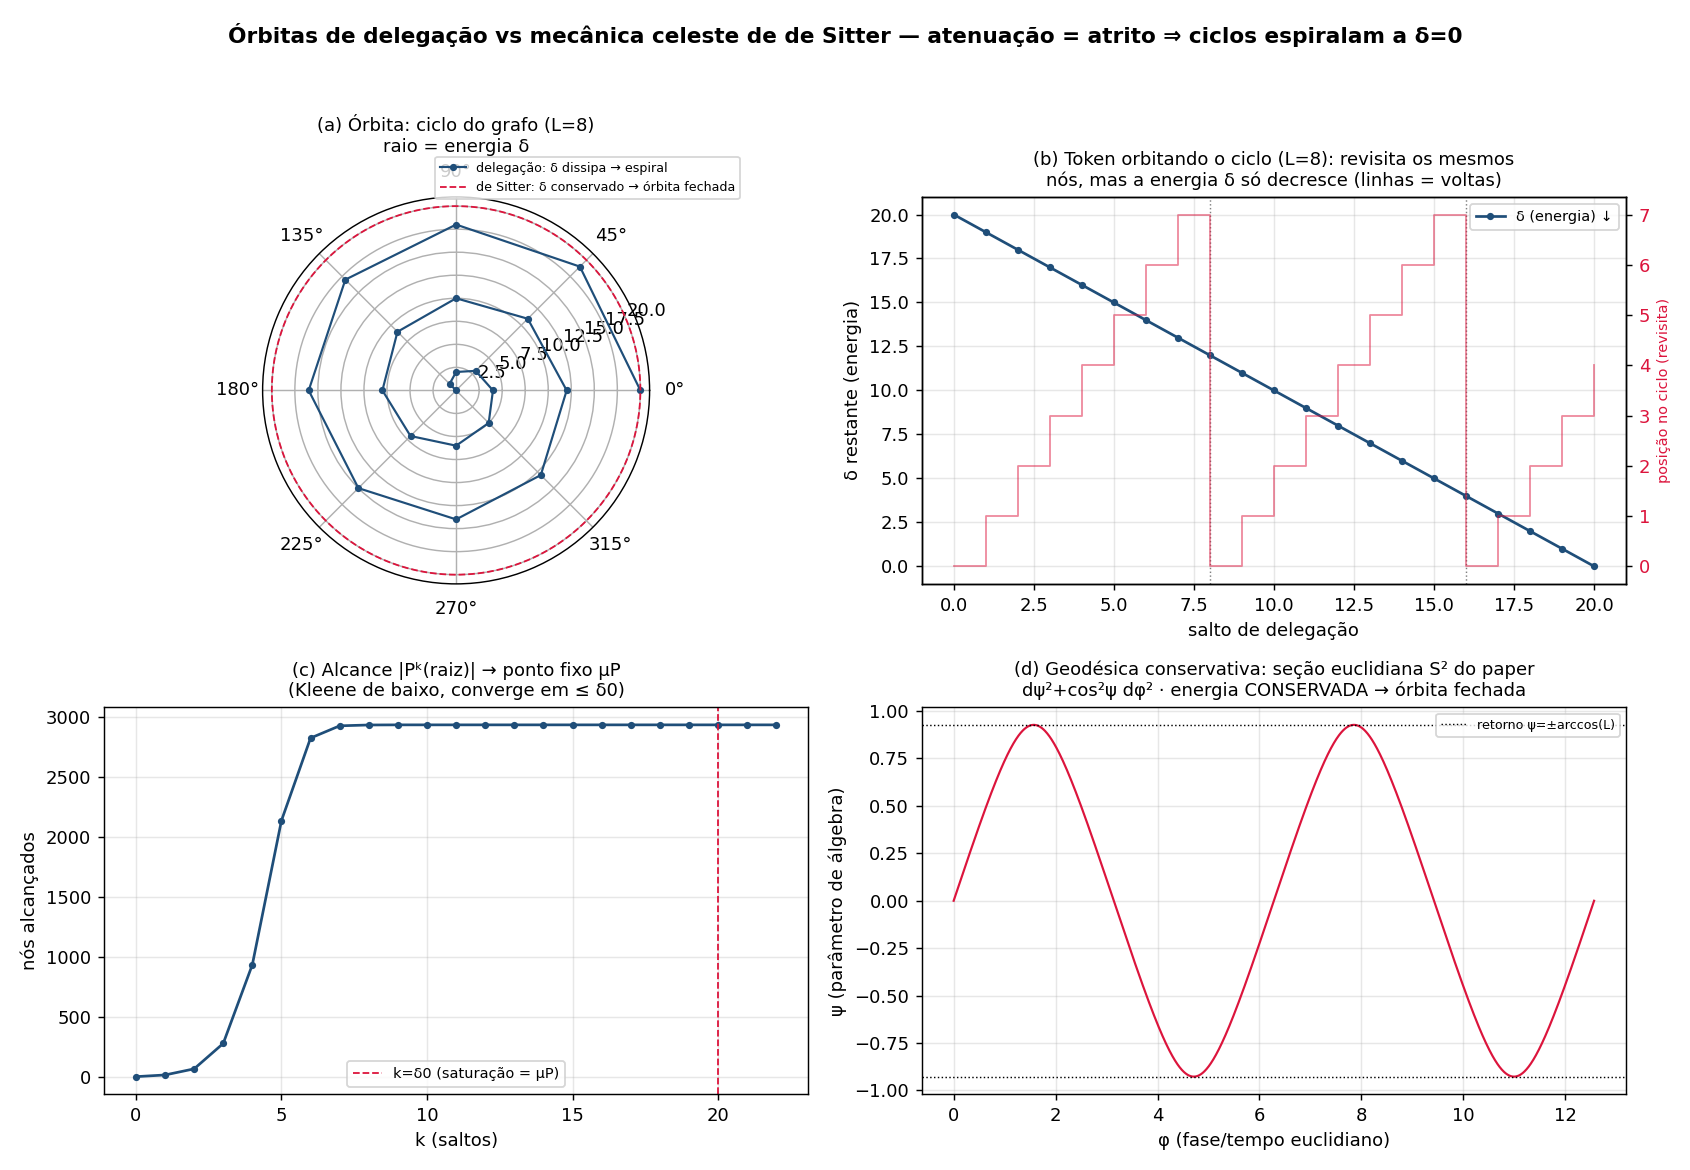
\includegraphics[width=\textwidth]{orbits/delegation_orbits.png}
  \caption{Órbitas de delegação \emph{vs} a geodésica conservativa. \textbf{(a)}
  A órbita de um ciclo do grafo: a delegação (azul) espirala para dentro porque
  $\dep$ dissipa, enquanto a de Sitter (vermelho) é um círculo de raio constante
  (energia conservada). \textbf{(b)} O token revisita os mesmos nós (a órbita),
  mas $\dep$ só decresce. \textbf{(c)} O alcance $|P^k(\mathrm{orig})|$ converge
  ao ponto fixo $\mu P$, saturando em $k\le\dep$ (Kleene de baixo). \textbf{(d)}
  A geodésica conservativa da seção euclidiana $S^2$ do paper: órbita fechada,
  energia conservada --- o contraponto sem atrito.}
  \label{fig:orbits}
  \end{figure}

  \begin{remark}[Não é identificação física, é analogia dinâmica]
  O caso conservativo (de Sitter/esfera) e o dissipativo (delegação) diferem
  \emph{exatamente} pelo termo de atrito $=$ atenuação. É essa dissipação que
  torna o sistema seguro a escala --- com ciclos e tudo, sem precisar de DAG.
  \end{remark}

  \begin{remark}[Duas leituras: matemática e observabilidade]\label{rem:leituras}
  Esta seção admite duas leituras. \textbf{Leitura A} (matemática): o sistema
  lembra uma dinâmica dissipativa em de Sitter. \textbf{Leitura B} (produto): o
  estado de autorização da empresa forma um \emph{universo observável}. Para um
  ERP, B talvez seja a mais valiosa --- administradores não leem provas de
  não-escalada, mas leem instantaneamente uma visualização em que a autoridade
  \emph{nasce numa estrela} (operador ou tenant), \emph{flui} pelo grafo,
  \emph{perde energia}, \emph{forma órbitas}, \emph{encontra horizontes} e
  \emph{produz regiões densas de poder}. As mesmas grandezas viram uma camada de
  observabilidade e auditoria: a \emph{massa autorizativa}
  $M(p)=\sum_{\kappa\in\mathrm{Hold}(p)}\dep_\kappa$ (concentração de poder), as
  órbitas (sinal organizacional --- ciclos administrativos indicam
  \emph{bypass} de governança), a \emph{curvatura} $C(p)$ (hubs e gargalos), o
  horizonte $\dep=0$ (``esta autorização termina aqui'') e os \emph{sinais
  vitais geométricos} (energia/alcance/diâmetro/n\textsuperscript{o} de órbitas)
  ao longo do tempo. A detecção de anomalia se dá pela \textbf{geometria do
  sistema}, não pelo conteúdo das permissões: conta comprometida, exfiltração
  ou reorganização deixam a \emph{mesma assinatura} --- a física sai do
  equilíbrio --- ainda que toda regra seja válida. Protótipo em
  \texttt{doc/orbits/authorization\_cosmos.py}.
  \end{remark}

  % ============================================================
  \section{Nível de campo: a delegação em de Sitter 4D}\label{sec:field}
  % ============================================================

  Até aqui a condição $c$ seleciona \emph{linhas}. Mas o CASL também restringe
  \emph{campos} (colunas): uma regra pode conceder ``ler \texttt{Customer.name,
  \,Customer.email}'' sem dar \texttt{Customer.document}. Isto é uma segunda
  dimensão.

  \begin{definition}[Capacidade a nível de campo]
  Seja $\F$ o conjunto de campos (de um subject). Uma capacidade ganha um
  \emph{conjunto de campos} $\varphi\subseteq\F$:
  $\kappa=(a,s,c,\varphi,\iota,\dep)$, com extent
  $\ext{\kappa}=\ext{c}\times\varphi\subseteq\R\times\F$. A autorização efetiva
  vive agora em $2^{\R\times\F}$.
  \end{definition}

  \paragraph{O \emph{lift} é de graça (a álgebra é agnóstica ao portador).} Tudo
  o que provamos --- deny-overrides (Prop.~\ref{prop:deny}), atenuação e
  não-escalada (Teor.~\ref{thm:noesc}), $\dep$ e o ponto fixo $\mu P$, a
  cosmologia (Seção~\ref{sec:orbits}) --- usou \emph{apenas} a estrutura de
  dioid booleano de $2^{X}$, \textbf{nunca} o portador $X$ específico. Trocar
  $X=\R$ por $X=\R\times\F$ não muda uma linha das demonstrações. A atenuação
  agora estreita \emph{dois} eixos independentes: $\ext{c'}\subseteq\ext{c}$
  (linhas) \emph{e} $\varphi'\subseteq\varphi$ (campos). O \emph{pushdown}
  projeta a condição no \texttt{where} (linhas) e o $\varphi$ no \texttt{select}
  (campos) --- o que a extensão RLS já faz com \texttt{fields}.

  \paragraph{A geometria sobe duas dimensões.} O espaço dinâmico do nível de
  linha era $\dS_2$ (Seção~\ref{sec:orbits}): a fase $t$ do fluxo de delegação
  mais a energia $\dep$ (o $\rho$). Os campos acrescentam suas \emph{direções}
  --- uma esfera $S^2$ de configurações de campo $(\alpha,\beta)$, à la as
  esferas de direções de álgebra do paper. A forma estática de de Sitter
  generaliza exatamente assim:
  \begin{equation}
    \dS_n:\quad ds^2=-\cos^2\!\rho\,dt^2+d\rho^2+\sin^2\!\rho\,d\Omega^2_{n-2},
    \label{eq:dSn}
  \end{equation}
  onde $(t,\rho)=(\text{fluxo, energia }\dep)$ e $d\Omega^2_{n-2}$ são as
  direções de campo. O nível de linha é \eqref{eq:dSn} com $n=2$ (a métrica do
  paper, $d\Omega_0$ trivial); o nível de campo com uma esfera de campo $S^2$ é
  $n=4$:
  \[
    ds^2=-\cos^2\!\rho\,dt^2+d\rho^2+\sin^2\!\rho\,(d\alpha^2+\sin^2\!\alpha\,d\beta^2).
  \]

  \begin{theorem}[de Sitter 4D suporta o nível de campo]\label{thm:dS4}
  A métrica \eqref{eq:dSn} com $n=4$ é um espaço de Einstein de curvatura
  constante --- de Sitter $\dS_4$ de raio $\ell=1$:
  \[
    R_{\mu\nu}=(n-1)\,g_{\mu\nu}=3\,g_{\mu\nu},\qquad R=n(n-1)=12.
  \]
  \end{theorem}
  \begin{proof}[Verificação]
  Cálculo do tensor de Ricci em \texttt{doc/orbits/desitter4d.py} (Christoffel
  $\to$ Riemann $\to$ Ricci), conferido numericamente em $12$ pontos (resíduo
  $\sim10^{-16}$), \emph{exatamente} a metodologia do paper. O caso $n=2$
  reproduz $\dS_2$ ($R_{\mu\nu}=g_{\mu\nu}$, $R=2$) como controle. Em geral,
  $k$ dimensões de campo dão $\dS_{2+k}$.
  \end{proof}

  \begin{remark}[A cosmologia se completa]
  O horizonte $\rho=\pi/2$ (energia $\dep$ esgotada, o quaternion do paper)
  continua sendo o fim de vida da órbita (Seção~\ref{sec:orbits}); a esfera de
  campo $\sin^2\!\rho\,d\Omega^2_2$ acopla as direções de campo à mesma energia.
  A autorização a nível de campo é, então, um universo $\dS_4$ em meio
  dissipativo --- a mesma física do nível de linha, com duas direções
  espaciais a mais. A escolha do nível (linha vs campo) é só a dimensão do
  cosmos; a segurança (atenuação, não-escalada, vida finita) é idêntica em
  qualquer $n$.
  \end{remark}

  % ============================================================
  \section{Ciclo de vida: revogação e expiração}\label{sec:lifecycle}
  % ============================================================

  Uma concessão não é eterna. Modelamos o seu \emph{ciclo de vida} como uma
  máquina de estados finita (FSM), separada da álgebra de avaliação: a álgebra
  diz \emph{o que} uma capacidade autoriza; a FSM diz \emph{se} ela está em
  vigor.

  \begin{definition}[Instância de concessão]
  Uma \emph{instância} é uma capacidade $\kappa$ acrescida de
  $(\mathrm{orig},\mathrm{par},\tau,\sigma)$: a \emph{origem} $\mathrm{orig}$
  (quem concedeu), o \emph{pai} $\mathrm{par}$ (a instância da qual foi
  atenuada, ou $\bot$ se intrínseca), a \emph{expiração}
  $\tau\in\mathbb{R}_{>0}\cup\{\infty\}$ e o \emph{estado}
  $\sigma\in\{\textsf{active},\textsf{suspended},\textsf{revoked},
  \textsf{expired}\}$. As arestas válidas (Definição~\ref{def:att}) já exigem
  $\tau_\kappa\le\tau_{\kappa_0}$: \textbf{um filho nunca sobrevive ao pai}.
  \end{definition}

  \begin{definition}[Avaliação filtra o ciclo de vida]
  Em $\mathrm{Hold}(p)$ e em $E_p(s,a)$ (Seção~3) contam \emph{somente} as
  instâncias \textbf{vigentes} no instante $t$: $\sigma=\textsf{active}$ e
  $\tau>t$. As demais não contribuem. Assim revogar/suspender/expirar uma
  concessão remove o seu extent da união sem tocar na álgebra.
  \end{definition}

  \begin{figure}[h]
  \centering
  \begin{tikzpicture}[
      >={Stealth[round]}, node distance=26mm,
      st/.style={draw,rounded corners,minimum width=20mm,minimum height=8mm,font=\small},
      term/.style={st,fill=black!6},
      lbl/.style={font=\scriptsize,text=black!70},
    ]
    \node[st,fill=blue!8] (active) {\textsf{active}};
    \node[st, left=of active] (susp) {\textsf{suspended}};
    \node[term, right=of active] (exp) {\textsf{expired}};
    \node[term, below=14mm of active] (rev) {\textsf{revoked}};
    \node[lbl, above=4mm of active] (start) {concede (atenuação)};
    \draw[->] (start) -- (active);
    \draw[->,transform canvas={yshift=2pt}] (active) -- (susp) node[lbl,midway,above]{suspende};
    \draw[->,transform canvas={yshift=-2pt}] (susp) -- (active) node[lbl,midway,below]{retoma};
    \draw[->] (active) -- (exp) node[lbl,midway,above]{$t\ge\tau$};
    \draw[->] (active) -- (rev) node[lbl,midway,right]{revoga};
    \draw[->] (susp) to[bend right=30] node[lbl,midway,left]{revoga} (rev);
  \end{tikzpicture}
  \caption{FSM do ciclo de vida de uma concessão. \textsf{revoked} e
  \textsf{expired} são terminais; só \textsf{active} contribui para a
  avaliação. \emph{Guard} das transições destrutivas (suspende/revoga): o ator
  deve ter autoridade sobre a instância (ser a origem, um ancestral na cadeia,
  ou $\Omega$).}
  \label{fig:fsm}
  \end{figure}

  \begin{theorem}[Revogação em cascata]\label{thm:cascade}
  Revogar uma instância $I$ revoga toda a sua descendência na floresta de
  derivação (as instâncias cuja cadeia de $\mathrm{par}$ passa por $I$). Após a
  cascata, nenhuma instância vigente foi atenuada de $I$.
  \end{theorem}
  \begin{proof}
  Pela Definição~\ref{def:att}, toda instância $J$ atenuada (direta ou
  transitivamente) de $I$ tem $I$ na sua cadeia de pais. A cascata é a travessia
  dessa floresta a partir de $I$, marcando \textsf{revoked}. Como
  $\textsf{revoked}$ é terminal e excluída da avaliação, nenhuma sobrevive.
  \end{proof}

  \begin{corollary}[Expiração cascateia sozinha]
  Como $\tau_{\text{filho}}\le\tau_{\text{pai}}$, ao expirar o pai
  ($t\ge\tau_{\text{pai}}$) todos os filhos já expiraram. A expiração não
  precisa de travessia --- o invariante de atenuação a propaga.
  \end{corollary}

  \begin{remark}[A FSM é o lugar certo; a avaliação não]
  A decisão de acesso permanece uma \emph{computação pura} (a álgebra de §3--§6).
  A FSM modela apenas o que é genuinamente \emph{stateful}: transições
  auditáveis e a cascata de revogação sobre a floresta de derivação. Os dois compõem sem se
  contaminar.
  \end{remark}

  % ============================================================
  \section{\emph{Enforcement}: \emph{pushdown} no \emph{data layer}}\label{sec:enf}
  % ============================================================

  A avaliação independe de $\dep$ (Seção~\ref{sec:dag}): basta empurrar
  $E_p(s,a)$ para o \texttt{where}. Numa leitura de subject $s$ pelo principal
  $p$,
  \[
    \text{retornado}=E_p(s,\texttt{read})\cap\ext{c_{\text{query}}} .
  \]
  Escritas validadas contra $E_p(s,a)$; o conjunto de campos restringe colunas.
  Concretamente: uma \emph{extensão do Prisma Client} ($\texttt{\$allOperations}$)
  que injeta $\bigcup$(grants) $\setminus\bigcup$(proibições) via \texttt{AND}.

  \begin{remark}[Onde $\dep$ é verificado]
  A intensidade é checada no \textbf{ato de delegar} --- quando um principal
  cria/atribui uma capacidade a outro, valida-se a atenuação
  (Definição~\ref{def:att}: condição $\subseteq$, $\dep'\le\dep-1$). A leitura
  de dados nunca consulta $\dep$. Isso mantém a extensão RLS simples e a
  auditoria concentrada no momento da concessão.
  \end{remark}

  \begin{remark}[Dois modos e o piso nativo]
  \texttt{shadow} computa e \emph{registra} onde negaria sem alterar o
  resultado; \texttt{enforce} aplica. \texttt{\$queryRaw} escapa da extensão de
  aplicação; por isso um teste-\emph{guardrail} barra \emph{raw} fora de uma
  \emph{allowlist} escopada, e a Fase~B adiciona \emph{Row-Level Security}
  nativa do PostgreSQL como piso duro.
  \end{remark}

  \appendix
  % ============================================================
  \section{Plano de implementação}\label{ap:plano}
  % ============================================================

  \textbf{Escopo (backbone).} A avaliação (\emph{pushdown} da união de
  capacidades detidas) já está implementada e testada
  (\texttt{condition-resolver.ts}, \texttt{prisma-rls.extension.ts}): ela
  \emph{independe} de $\dep$, logo vale desde já. A camada de \emph{delegação}
  com $\dep$ (grafo, atenuação) entra com o multi-org; o campo e o primitivo de
  atenuação são preparados agora.

  \paragraph{A1. Capacidade carrega $\dep$.}
  Adicionar \texttt{propagationDepth Int?} a \texttt{AccessRule}
  (\texttt{null}$=\infty$; $0=$ não re-delegável) e a \texttt{RuleInput}. Migração
  nullable, retrocompatível (regras atuais $=\infty$).

  \paragraph{A2. Primitivo de atenuação (testado).}
  \texttt{access/delegation.ts}: \texttt{attenuatedDepth(holder, proposed)}
  ($\infty-1=\infty$; exige \texttt{holder}$\ge1$; \texttt{proposed}$\le$
  \texttt{holder}$-1$) e \texttt{canDelegate}. Verificado no serviço de
  concessão (criar regra / atribuir perfil), \emph{não} na leitura.

  \paragraph{A3. Avaliação (já feita).}
  \texttt{condition-resolver.ts}: $E_p=$ união dos grants $\setminus$ proibições,
  sob o escopo herdado. \texttt{prisma-rls.extension.ts}: injeção no
  \texttt{where}, OR nos grants, fail-closed, guarda de \emph{create}
  cross-escopo, modos \texttt{shadow}/\texttt{enforce}. Mapa
  \emph{Subject}$\leftrightarrow$\emph{model}; \emph{registry} via DMMF.

  \paragraph{A4. \emph{Wiring}.}
  \texttt{TenantContext} carrega regras + escopo + \texttt{rlsMode};
  \texttt{PrismaService} vira \emph{Proxy} por-\emph{request} com client
  estendido; \texttt{PoliciesGuard} reusa as regras do contexto.

  \paragraph{A5. Testes (por funcionalidade --- exigência central).}
  \texttt{condition-resolver.spec}, \texttt{prisma-rls.extension.spec} (por
  subject/model), \texttt{delegation.spec} (atenuação/$\dep$),
  \texttt{ability.contract.spec} (matriz dos perfis), \emph{guardrail} de
  \emph{raw}. Regra de projeto: nenhuma capacidade/perfil novo sem teste.

  \paragraph{A6. Gate na CI.}
  \emph{job} \texttt{test} (\texttt{npm ci} + \texttt{prisma generate} +
  \texttt{npm test}); \texttt{deploy} com \texttt{needs: test}.

  \paragraph{A7. \emph{Rollout}.}
  \texttt{RLS\_MODE=shadow} $\to$ \texttt{enforce}. Fase~B: RLS nativa do
  PostgreSQL como piso duro.

  \paragraph{A8. Ciclo de vida (FSM) --- Seção~\ref{sec:lifecycle}.}
  \texttt{AccessRule} ganha \texttt{state} (\textsf{active}/\textsf{suspended}/
  \textsf{revoked}/\textsf{expired}), \texttt{expiresAt DateTime?}
  (\texttt{null}$=\infty$) e \texttt{parentId} (auto-relação para a cascata).
  A avaliação passa a filtrar \texttt{state='active' AND (expiresAt IS NULL OR
  expiresAt > now())} --- some uma cláusula na carga das regras, a álgebra não
  muda. Atenuação de $\tau$ no \emph{grant-check} (espelho de
  \texttt{attenuatedDepth}). Transições auditadas; \emph{guard} = autoridade
  sobre a instância.

  \emph{Revogação a escala.} A cascata por \texttt{parentId} (CTE recursiva)
  custa $O(\text{tamanho da subárvore})$ --- caro ao revogar uma raiz com
  $10^5$ descendentes. Como a floresta de derivação é \emph{imutável} (o pai de
  uma concessão nunca muda) e bem-fundada (Lema~\ref{lem:energy}), materialize
  \texttt{rootGrantId} (a autoridade intrínseca de origem) e/ou um
  \texttt{path} (\emph{materialized path}) no momento da concessão. Revogar uma
  raiz vira \texttt{UPDATE ... WHERE rootGrantId = \$1} (um \emph{index scan},
  $\approx O(1)$ amortizado); revogar uma subárvore qualquer,
  \texttt{WHERE path LIKE \$1 || '\%'}. A CTE recursiva fica como caminho de
  fallback.

  \end{document}
